\documentclass[../main.tex]{subfiles}
\begin{document}

In this chapter, we are interested in giving a review of the literature on how to build relational structures automatically. While reviewing pieces of work, we are interested in two aspects: one is the pipeline used to build the relational structure itself, which comprises the mathematical models and algorithms applied to this end, along with their assumptions. If these assumptions are met in our model, then their pipeline or a subset of it could be useful.
\par Additionally, the second aspect of interest are the goals and components of the target relational structure, i.e. the entities and relationships the authors modelled. Discovering links between pairs of bird species is different from segmenting vowel sounds in human speech, for example. Although these differences will probably be reflected in different pipelines, understanding them is key in order to produce a pipeline that will yield better results for our work.
\par However, limiting ourselves to works focusing exclusively on this task might be too restrictive: results from bird classification, clustering and detection could also prove useful for our project. For example, feature extraction is common to all tasks, and state-of-the-art feature extraction is mandatory in order to achieve better results. Therefore, whenever relevant, works on these tasks will also be cited in this review.
\par This chapter is presented as follows: firstly, a general overview of pipelines for building relational structures is given; afterwards, we present a review of feature extraction methods used in acoustic signals; algorithms for building relational structures are reviewed next; finally, a discussion on how the referenced methods are relevant a working pipeline for our scenario is presented.

\section{Relational structures and pipelines}\label{general_pipeline}
A relational structure is one that shows links between objects. In this work, we will assume these links to be a binary relations $R$ over a single set $X$, i.e. $R \subseteq X \times X$. One way of representing such relations is a square matrix $A$, called \emph{adjacency matrix}, such that $A \in \mathbb{R}^{n \times n}$, where $n =\left\vert{X}\right\vert$.
\par In real life, information about objects can be represented as a relational structure. As the number of objects grows large, specific subsets of $R$ may present an increasingly "complex" topology. "Complex graphs" (as they are commonly called in the literature) and how to identify them have been extensively discussed in the field. In \cite{Kim2008}, the authors give a narrowed definition for complex graph, which we adapt as follows:
\theoremstyle{definition}
\begin{definition}{Complex graph}. One such that its topological features deviate from random graphs. In other words, a graph that contains many different subgraphs.
\end{definition}
\par A problem that has attracted attention in recent years is community detection. Given a graph $G = (X, E)$ depicting a relation between pairs of objects in $X$, community detection can be seen as a problem of clustering over $X$, i.e. partitioning the vertices $X$ in such a way that the edges between those in different clusters "are comparatively fewer than those between those belonging to the same cluster" \cite{Fortunato2010}. 
\par Clustering is the task of "grouping or segmenting a collection of objects into subsets or clusters, such that those within each cluster are more closely related to one another than objects assigned to different clusters" \cite{hastie2008}. An example of clustering for the 2-dimensional case can be seen in \ref{clustering}.
\begin{figure}[ht]
\centering
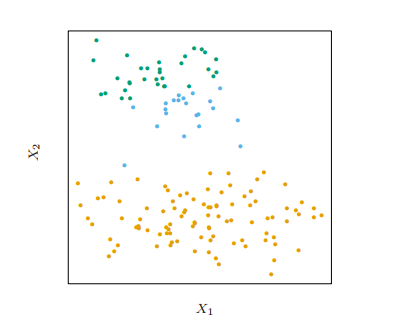
\includegraphics{clustering}
\caption{Simulated data in the plane, clustered into three classes. Image taken from \cite{hastie2008}.}
\label{clustering}
\end{figure}
\par Therefore, performing clustering requires computing the \emph{closeness} of elements in the set of objects $X$. Proximity, closeness, similarity or dissimilarity, all refer to \emph{distance functions} or \emph{metrics}. 
\theoremstyle{definition}
\begin{definition}{Metric}.
\label{def_metric}
A non-negative function $d$ satisfying:
\begin{enumerate}
\item Triangle inequality. $d(x, z) \leq d(x, y) + d(y, z) $
\item Symmetry. $d(x, y) = d(y, x)$
\item $d(x, x) = 0$
\item $d(x, y) = 0 \iff x = y$
\end{enumerate}
\end{definition}
\par Thus, defining a metric requires knowledge about what kind of objects we are grouping. In Machine Learning in particular, we will also be concerned by how we transform data into objects for which we can define a metric. This process, called \emph{feature extraction}, consists in "deriving features from raw data that can be used as input for a learning procedure" \cite{hastie2008}. The goal is to use domain knowledge to extract features that will reduce redundancy in raw data and highlight distinguishing characteristics, thus optimising the learning procedure in both, correctness and performance \cite{Bishop2006}. 
\par By working our way backwards, we have implicitly defined a general pipeline to be followed to build relational structures: the algorithms that do so, require the definition of a metric between objects. These objects will be the vectors or features extracted from each object of interest. A diagram depicting this procedure is shown in \ref{pipeline}.
\begin{figure}
\centering
\begin{tikzpicture}[node distance=2cm]
\node (start) [startstop] {Start};
\node (in1) [io, below of=start] {Raw data};
\node (pro1) [process, below of=in1] {Feature extraction};
\node (in2) [io, below of=pro1] {Features};
\node (pro2) [process, below of=in2] {Compute similarity};
\node (in3) [io, below of=pro2] {Pairwise proximity};
\node (pro3) [process, below of=in3] {Build relational structure};
\node (out1) [io, below of=pro3] {Relational structure};
\node (stop) [startstop, below of=out1] {Stop};
\draw [arrow] (start) -- (in1);
\draw [arrow] (in1) -- (pro1);
\draw [arrow] (pro1) -- (in2);
\draw [arrow] (in2) -- (pro2);
\draw [arrow] (pro2) -- (in3);
\draw [arrow] (in3) -- (pro3);
\draw [arrow] (pro3) -- (out1);
\draw [arrow] (out1) -- (stop);
\end{tikzpicture}
\caption{A general pipeline to build relational structures.}
\label{pipeline}
\end{figure}
\par We can now tackle the rest of this literature review as stages that we can put together in order to build relational structures. We will first give an overview of general aspects of birdsong in section \ref{birdsong_review}, aiming to present in a structured manner the data to be analysed in this work. After, we will dedicate a section for each of the processes comprised in the general pipeline. Section \ref{features_review} presents different procedures to extract features from birdsong automatically. Later, section \ref{metrics_review} gives a definition of metrics frequently used in the literature. Finally, section \ref{algorithms_review} gives an overview of algorithms used to generate relational structures from input vectors and metrics.

\section{General aspects of birdsong} \label{birdsong_review}
In this section, we present the concept of birdsong from a biological perspective. We will address this by giving relevant information on the acoustic structure of birdsong, and how it differs from its counterpart, bird calls. Moreover, we also touch on the social and behavioural functions of birdsong and its relation to human speech. Finally, we discuss some arguments regarding the evolution of birdsong through time.
\par There are two ways of acoustic communication among birds: songs and calls. The former "resemble speech in that they are acoustically complex sequences of stereotyped vocal gestures, lasting from seconds to minutes" \cite{Snowdon2013}. On the other hand, bird calls are shorter, consonant-like sounds whose "contribution to nature's music is minimal" \cite{Marler2004}. 
\par From a functional perspective, birdsong is used to defend territories and for mate attraction or competition \cite{Berwick2013} \cite{Naguib2014}, whereas calls are more intimately related to "issues of life and death, such as: predator alarm, the announcement and exchange of food, and the maintenance of social proximity and group composition and integration" \cite{Marler2004}.
\par Birdsongs and bird calls are also different structurally. Biologists have proposed a hierarchical structure of birdsong: a single song is composed of multiple motifs or patterns, each of which is composed of syllables \cite{Snowdon2013}. This structure can be observed in figure \ref{fig_birdsong_structure}. Bird calls, on the other hand, "are often short, monosyllabic, with simple frequency patterning, often delivered in what often appears to be a disorderly fashion" \cite{Marler2004}. Thus, bird calls often lack the hierarchical structure and repetitive patterns that are so distinctive of birdsong. An example of this can be seen in figure \ref{fig_birdcall}.

\begin{figure}[t]
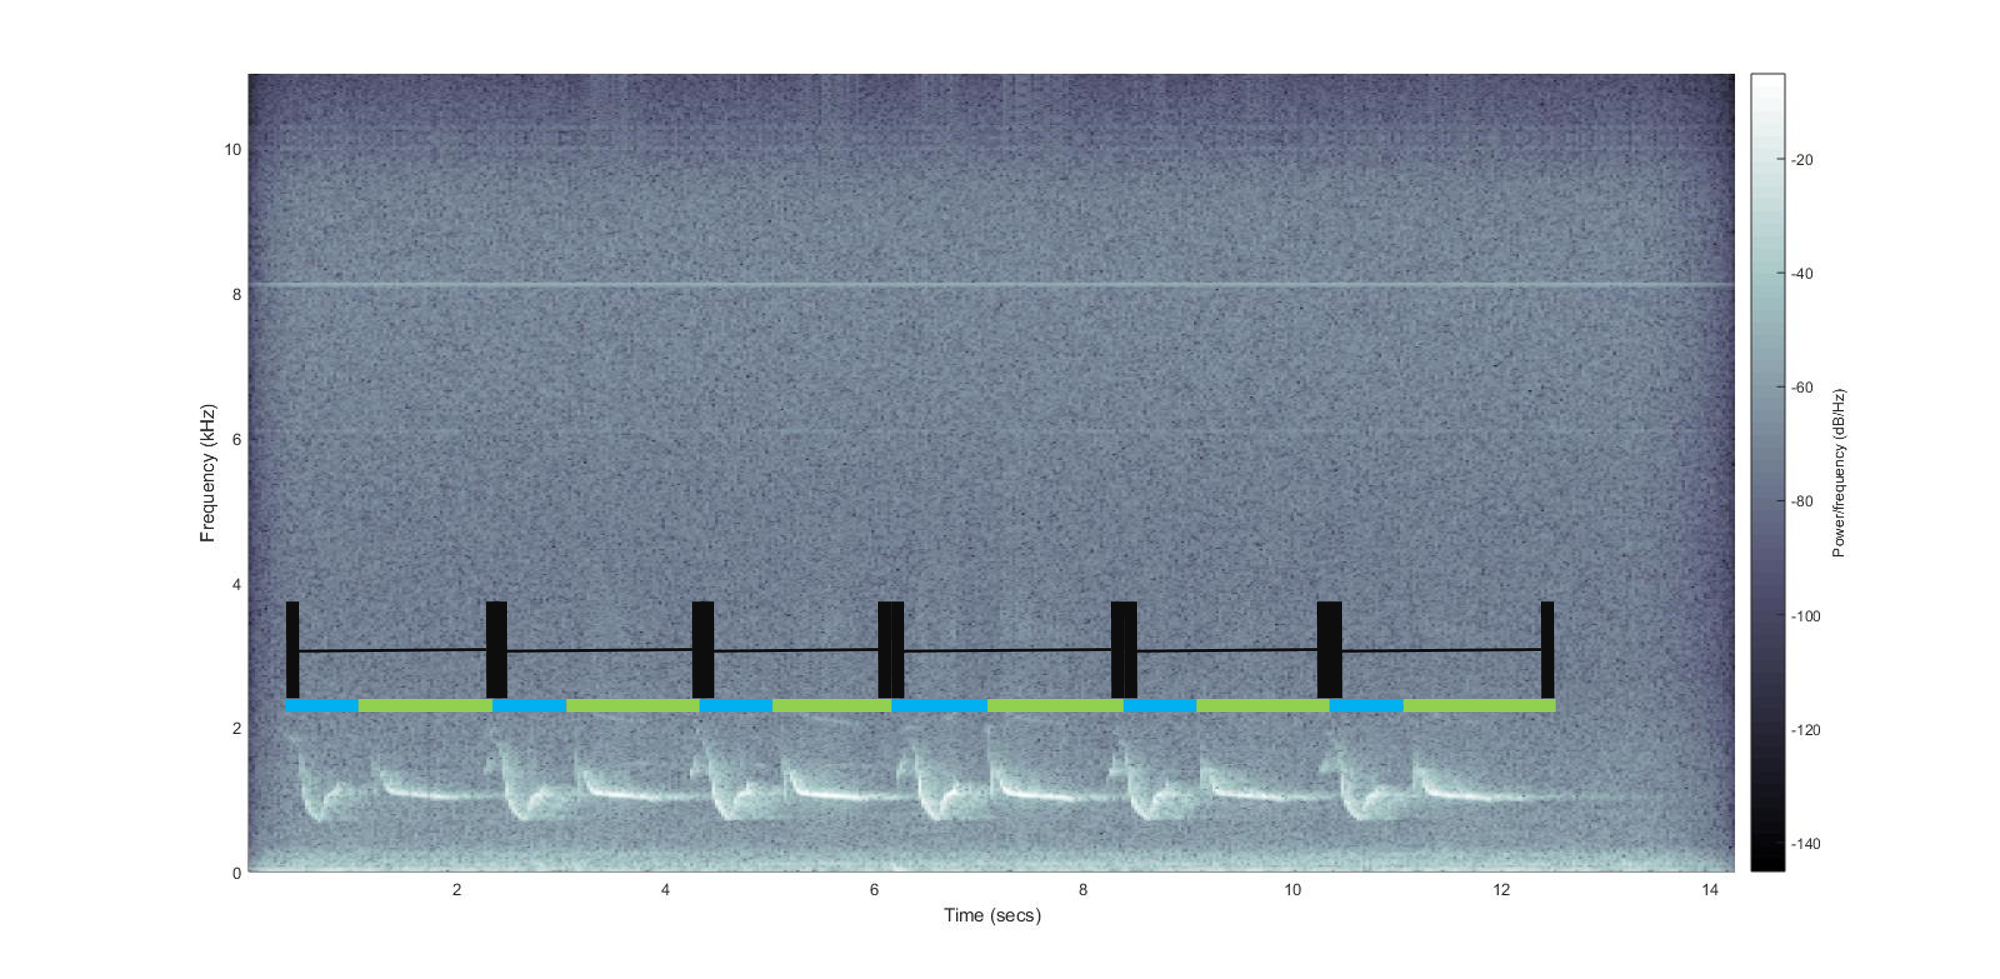
\includegraphics[width=\textwidth]{birdsong_structure}
\caption{Spectrogram from a birdsong recording of the species \emph{Periparus ater}. The thick blue and green bars represent syllables, and the black boxes represent a motif.}
\label{fig_birdsong_structure}
\end{figure}

\begin{figure}[t]
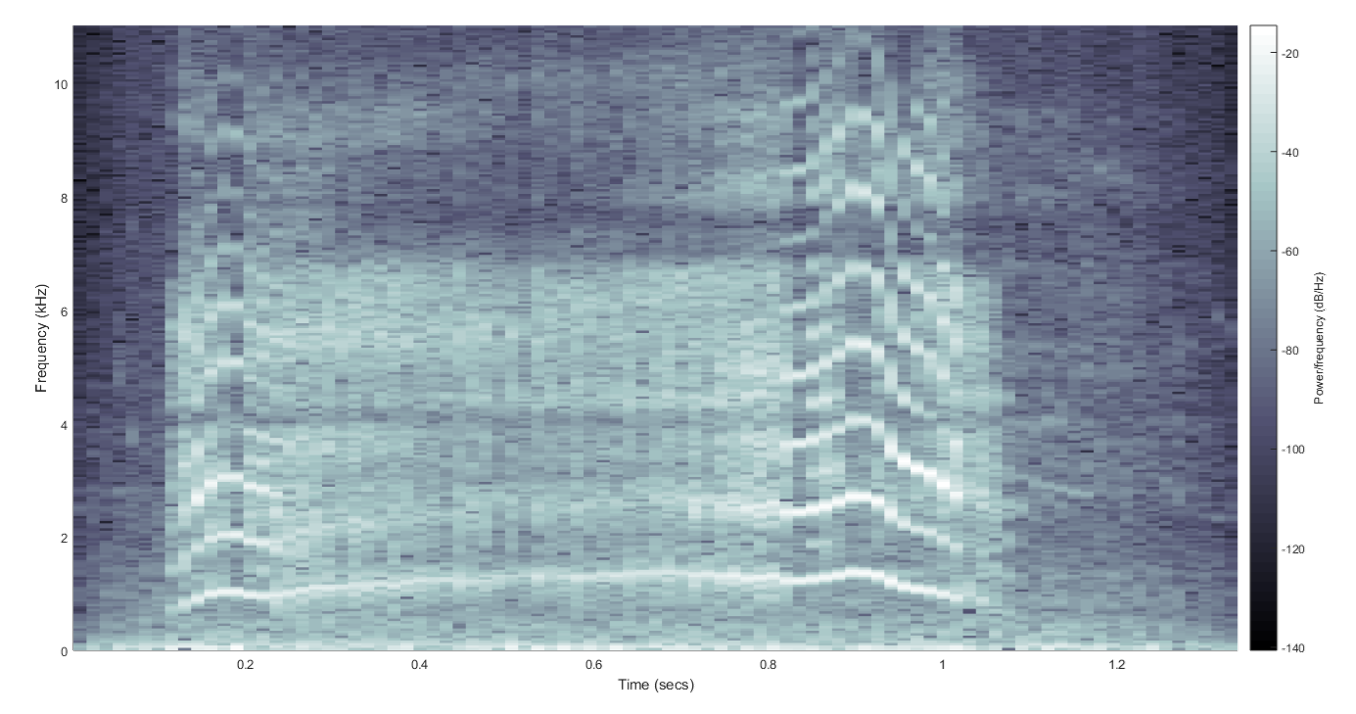
\includegraphics[width=\textwidth]{birdcall}
\caption{Spectrogram from a bird call recording of the species \emph{Vanillus vanillus}.}
\label{fig_birdcall}
\end{figure}

\par In this work, we will be concerned exclusively with birdsong examples. Now that we have compared both types of bird communication, we will focus only on birdsong. The remaining of this section will present more relevant features of birdsong and its association with human speech and evolution.
\par Biologists support the idea that birdsong is learnt by imitation of parent birds \cite{Berwick2013}, i.e. young birds copy many elements of elder birds to produce birdsong. Moreover, the patterns that can be produced by birds can take a long time to master, since birdsong depends on many factors, for example \cite{Naguib2014}: 
\begin{itemize}
\item Some motifs are longer than others, thus mastering them takes longer.
\item Some songs are only produced at a particular time of the day or season of the year.
\item Since one function of birdsong is mating, some songs may only be produced during the birds' fertility period.
\item The energy requirement varies among different songs.
\end{itemize}
\par The fact that birds learn to sing by imitating elder birds is a trait that has caught attention among the field scholars, due to its close relation to how humans learn to speak (by imitation as well). This is not the only similarity between both scenarios: both, birdsong and human language "involve complex, patterned vocalisations" \cite{Berwick2013} \cite{Naguib2014}. The similarity between birdsong and human speech is also related to the auditory system of birds and humans: both hear best between 2 and 5 kHz, unlike other models of animal auditory processing \cite{Snowdon2013}. Furthermore, the bird auditory system can hear frequencies as high as 10kHz, and its human counterpart can do so up to 20kHz \cite{Snowdon2013}.
\par However, biologists consider human speech to be much more complex lexically and semantically \cite{Berwick2013}, i.e. whereas birdsong has two very clear purposes, human speech serves to many more. These functions are closely tied to the highly structured syntactic structures of natural language. Another way to present this point is: the phonetic complexity of both means of communication is not what makes them most distinguishable (both have syllables that make up words), but the idea that human speech adds further levels of abstraction by proceeding to assemble words into sentences, and sentences into full discourses. The morphological, syntactic and semantic complexities of human speech are virtually absent from birdsong. Nevertheless, a strong link still exists in the phonetic abstraction of language.
\par At present, we could make yet another analogy between natural language and birdsong: if human languages have evolved and diversified over time due to sociological and environmental phenomena, how could a similar theory be developed for birdsong, assuming this were even possible? \cite{Cate2004} gives an account of this work stating that past researchers were skeptical about this theory, given that closely related species can diverge strongly in vocal features, just as much as how non-related species could converge in their vocal features due to environmental pressure. The former is more common than the latter, and it occurs often due to acoustic changes occurring in a particular generation, and carried over to the future. Additionally, birds that migrate might be pushed to change the way the sing (or call) due to the presence of new threats. In fact, \cite{Marler2004} states that the loss of natural habitats may actually leave us forever with unanswered questions, precisely due to the missing information that would permit us to trace back the evolution of birdsong.
\par To conclude this section, we point out that more recent research has supported the idea that there is still sufficient information to perform bird species classification \cite{Naguib2014}. Certainly, this is not the same as building a relational structure of bird species, and the arguments above could imply that there is no theoretical guarantee (at least from the biological perspective) that one such relation could exist. However, there is still no guarantee from a statistical or computational perspective that this is indeed the case, and thus Machine Learning becomes relevant to give an opinion on the matter from a mathematical perspective.

\section{Feature extraction procedures for birdsong} \label{features_review}
In this section, we give an account of different birdsong feature extraction techniques used in the literature. Most of these techniques rely on extracting information from the signal in the frequency domain, i.e. if we let a birdsong recording (or a portion of it) be a function of time, namely $x(t)$, then we can take it to the frequency domain and analyse it there. 
\subsection{The Fourier Transform and the FFT algorithm} \label{subsection_fft}
\par One widespread way of performing this domain shift is given by the Fourier transform \cite{Weisstein2015}, defined as:
\theoremstyle{definition}
\begin{definition}{Fourier Transform}.
Given a function $x(t)$, its Fourier transform $X(s)$ is defined as:
\begin{align*}
X(s) = \int_{-\infty}^{\infty}x(t)\mathrm{e}^{-2\pi ist}dx
\end{align*}
\end{definition}
\par We can also define a discrete version of this operation:
\begin{definition}{Discrete Fourier Transform}.
Given a discrete function $\{x_n\}$, its Fourier transform $\{X_k\}$ is defined as:
\begin{align*}
X_k = \sum_{n=0}^{N-1}x_n\mathrm{e}^{-2\pi i\frac{kn}{N}}
\end{align*}
\end{definition}
\par By far the most efficient way to perform the latter is the Fast Fourier Transform (FFT), which runs in $\mathcal{O}(N\log{N})$ \cite{Smith2011}. There are several versions of this algorithm, but one of the most well-known in the literature is the Cooley-Tukey algorithm, described by the eponymous authors \cite{Cooley1965}, \cite{Weisstein2015}. Its general strategy is to use intermediate results in a divide-and-conquer fashion in order to decrease the total number of operations \cite{Weisstein2015}, and it achieves so thanks to the Danielson-Lanczos Lemma:
\begin{lemma}
\emph{Danielson-Lanczos Lemma.} The DFT expansion $\{X_k\}$ of a discrete function $\{x_n\}$ can also be expressed as:\\
\begin{align*}
X_k &= \sum_{j=0}^{N/2-1}\mathrm{e}^{-2\pi i\frac{kj}{N/2}}x_{2j} + W^n\sum_{j=0}^{N/2-1}\mathrm{e}^{-2\pi i\frac{kj}{N/2}}x_{2j+1}\\
&=F^e_k + W^kF^o_k \\
\text{with } W &= \mathrm{e}^ {\frac{-2\pi i}{N} }
\end{align*}
\end{lemma}
\par This is merely regrouping the addition terms as two subadditions, one along the odd-numbered indices, and one along the even-numbered indices. Moreover, by periodicity of the DFT:
\begin{align*}
F^e_k &= F^e_{k+N/2}\\
F^o_k &= F^o_{k+N/2}\\
\mathrm{e}^ {\frac{-2\pi ik}{N} } &= -\mathrm{e}^ {\frac{-2\pi i(k+N/2)}{N} }
\end{align*}
\par This enables us to reformulate the calculation of $X_k$ as:
\begin{align*}
X_k = F^e_k + W^kF^o_k\\
X_{k+N/2} = F^e_k - W^kF^o_k
\end{align*}
\par These reformulations reduce the calculations per recursion to nearly half of the original number, thus resulting in a much better performing procedure. More specific details of this algorithm are beyond the scope of this work, but can be consulted in \cite{Smith2011} and \cite{Cooley1965}.
\par Having discussed the transformation of signals in the time domain into signals in the frequency domain, we are now prepared to set forth different methods of feature extraction.

\subsection{Mel Frequency Cepstral Coefficients (MFCC)} \label{subsection_mfcc}
\par This technique is one of the most widely used in human speech recognition \cite{Jurafsky2009}, \cite{Chou2008a}, \cite{Stowell2014}. It consists in representing the spectral envelope of a frame (a portion of a signal) by analysing its Mel-frequency \emph{cepstrum}. This is done for as many overlapping frames of equal length (around 20-50 milliseconds) that can be extracted from the original signal. The Mel scale is a frequency scale created to simulate how the human ear perceives sounds \cite{Sludge2000}. Its main premise is that human ear perception of pitch is linear below 1 kHz and logarithmic above. In other words, from 1 kHz, the same amount of energy is distributed along longer ranges of frequencies. This results in the human ear having a poorer performance distinguishing very high frequencies.
\par Hertz can be mapped to Mels by the following:
\begin{align*}
F_{\text{mel}} = 1127 \log{(1 + \frac{F_{Hz}}{700})}
\end{align*}
\theoremstyle{definition}
\par We now present the general (scale-independent) definition of the cepstrum, adapted from \cite{Gutierrez-Osuna2009}:
\begin{definition}{Cepstrum} \label{def_cepstrum}
The cepstrum $\V{c}$ of a discrete time signal $\V{x}$ is defined as the Inverse Discrete Fourier Transform (IDFT) of the log-magnitude of the frequency spectrum of $\V{x}$. In other words:
\begin{align*}
\V{c} = \mathcal{F}^{-1}\{\log{(\abs{\mathcal{F}\{\V{x}\}})}\}
\end{align*}
\end{definition}
\par Note that the absolute value $\abs{\mathcal{F}\{\V{x}\}}$ is the square root of the spectral energy of $\V{x}$, which is given by $E(\V{x}) = \abs{\mathcal{F}\{\V{x}\}}^2$. By using the knowledge from the Mel-scale, we can introduce the Mel-frequency cepstrum. The main difference between this and the one from definition \ref{def_cepstrum} is that we compute the magnitude of the spectrum in Mel-scale, rather than in Hertz. Given that the Mel-scale was introduced to model how the human ear detects pitch, this new estimate would show how energy in different \emph{critical bands} of frequencies is being detected by humans. A critical band is a range of frequencies centered around \emph{critical frequencies}, which are distributed according to the Mel-scale, i.e. uniformly before 1 kHz, and exponentially onwards \cite{Gutierrez-Osuna2009}. The length of this range is called the \emph{bandwidth} of the band.
\par In order to estimate the magnitude of the spectrum in Mel-scale, we compute the magnitude of the original frequency spectrum in Hertz and weight it by means of triangular filters along the frequency axis. Each filter corresponds to one critical band, is centered in a critical frequency and the length of its base corresponds to the bandwidth of the critical band, as pictured in figure \ref{mel_energy}.


\begin{figure}[t]
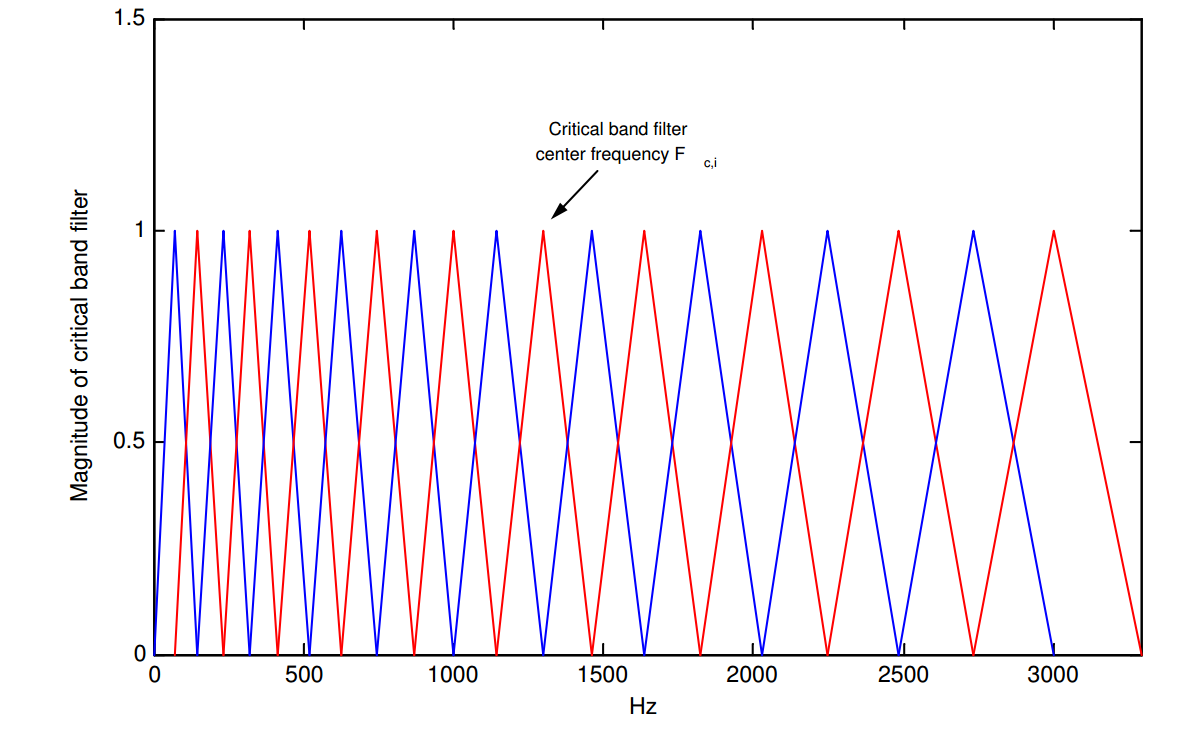
\includegraphics[width=\textwidth]{mel_energy}
\caption{Triangular frequencies to compute the spectral energy in the Mel scale. Picture taken from \cite{Sludge2000}.}
\label{mel_energy}
\end{figure}

\par Then, we continue with the steps described in definition \ref{def_cepstrum}. The result is called Mel-cepstrum and the MFCC are the first $k$ elements of the result. In practice, normally 13 coefficients are taken after using between 20 and 40 triangular filters \cite{Gutierrez-Osuna2009}. However, more recent research has shown that computers now have enough resources to use the full Mel spectrum, rather than just taking the first coefficients \cite{Stowell2014}. Furthermore, MFCC tend to be enhanced with the so-called \emph{delta features}, which represent the rate of change of the MFCC sequence over time \cite{Muda2010} \cite{Lyons2014}. 
\begin{definition}{Delta features.} \label{def_delta_mfcc}
Given a sequence of coefficients $\V{c}$, its delta features are given by:
\begin{align*}
\Delta_t = \frac{\V{c}_{t+1} - \V{c}_{t-1}}{2}
\end{align*}
\end{definition}
\par Similarly, \emph{double delta features} (or acceleration) can be computed by taking the delta features of the delta sequence. 
\par In \cite{Stowell2014}, an analysis of the performance of both, raw Mel spectra and MFCC is presented and compared against other feature extraction procedures when used to characterise birdsong. The conclusion is that, although standard for human speech, there is no proof that this should be the standardised feature extractor for birdsong. The authors present unsupervised feature learning as an alternative that could be more accurate, but call for further benchmarking to be done before coming to an absolute conclusion.

\subsection{Spherical k-means} \label{subsection_spherical}
This is an unsupervised approach to feature learning that consists in finding a normalised spanning set of $K$ vectors for the training dataset. The algorithm was first proposed by \cite{Coates2012}, first used for audio in \cite{Dieleman2013} and in particular for birdsong in \cite{Stowell2014}. It is a modification of the well-known K-means algorithm, where the main difference consists in assigning each datum to the cluster whose centroid produces the minimum cosine distance.
\begin{definition}{Cosine distance} \label{def_cosine_distance}
The cosine distance between two vectors $\V{x}$ and $\V{y}$ separated by an angle $\theta_{\V{x}, \V{y}}$ is given by:
\begin{align*}
d(\V{x}, \V{y}) &= 1 - \cos{(\theta_{\V{x}, \V{y}})}\\
&= 1 - \frac{\V{x} \cdot \V{y}}{\norm{\V{x}}\norm{\V{y}}}
\end{align*}
\end{definition}
\par Moreover, each centroid is normalised at every iteration of the algorithm. The result is a normalised spanning set that displays the directions of greater concentration of data, as depicted in figure \ref{fig_spherical}.

\begin{figure}[t]
\centering
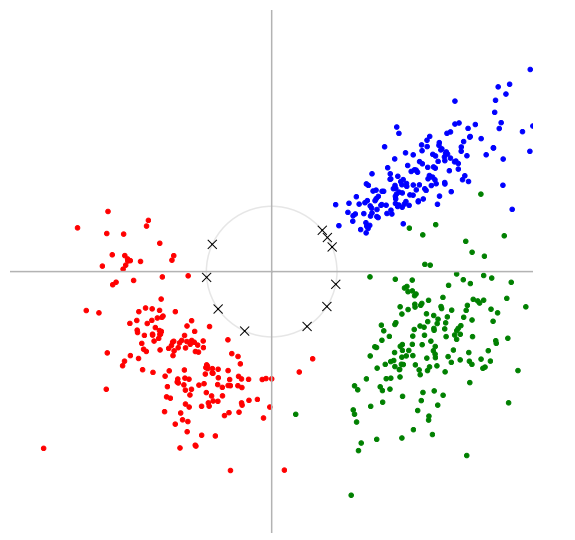
\includegraphics[width=80mm]{spherical}
\caption{Spherical k-means applied to artificial data generated from 3 different 2D-gaussians. The marks represent each of the normalised centroids. Image taken from \cite{Stowell2014}.}
\label{fig_spherical}
\end{figure}
\par The dot product of each datum $\V{x}_j$ with each of the vectors $\V{b}_i$ in the spanning set can be used as features $\V{x}^*_{i,j}$ for a learning procedure, with dimensionality equal to $K$. That is, let $\V{B}$ be the matrix whose rows are the vectors in the spanning set found by spherical k-means, then the new features are given by $\V{x}^*_j = \V{Bx}_j$. In \cite{Stowell2014}, spherical k-means is used as an unsupervised feature extraction procedure for birdsong recordings: the authors used Mel spectral frames (with 40 entries, as described in \ref{subsection_mfcc}) as input to the algorithm. As proposed in \cite{Dieleman2013}, all frames were normalised in length and preprocessed using PCA-whitening. More details of this procedure can be found in \cite{Stowell2014} and \cite{Dieleman2013}.

\subsection{Wavelets} \label{subsection_wavelets}
In this subsection, we give a brief overview of wavelets. This signal analysis technique has been used to analyse birdsong, showing "better results than MFCC" \cite{Chou2009}. Wavelets are an alternative to the Short-Time Fourier Transform (STFT), discussed in subsection \ref{subsection_mfcc}, under the argument that wavelets give better quality results because "they are localised in time and space". This last phrase means that, whereas a small change in the Fourier Transform of a function will produce changes everywhere in its time domain representation (i.e. the FT is only localised in frequency), this is not true for wavelets, since they are localised in both domains \cite{Vidakovic1991}.
\par To expand on this concept, we first introduce orthogonal wavelets.
\begin{definition}{Orthogonal wavelets.} \label{def_onwavelets}
A function $\psi\in L^2(\mathbb{R})$ is called an orthogonal wavelet if the family $\{\psi_{j,k}\}$ is an orthonormal basis for this $L^2(\mathbb{R})$, where each $\psi_{j,k}(t) = 2^{j/2}\psi(2^jt-k)$ and $j, k \in \mathbb{Z}$.
\end{definition}
\par The definition for each $\psi_{j,k}(t)$ arises from the ideas of \emph{binary dilation} and \emph{dyadic translation}: each function has the same shape as the original $\psi(t)$, but has been scaled and translated so as to cover as much as possible from the real line \cite{Chui1992}. 
\par The simplest example of an orthogonal wavelet is given by the Haar function, $\phi_H$ \cite{Chui1992}:
\begin{displaymath}
   \psi_H(t) = \left\{
     \begin{array}{lr}
      1 & 0 \leq t < 1/2 \\
      -1 & 1/2 \leq t < 1 \\
      0 & \text{otherwise} 
     \end{array}
   \right.
\end{displaymath}
\par Now, let $x(t)$ be a signal that belongs to the Hilbert space of square integrable functions, $L^2(\mathbb{R})$ with $\{\psi_{j,k}(t)\}$ as one of its bases. Then $x(t)$ can be expanded as an infinite linear combination:
\begin{align*}
x(t) = \sum_{j,k=-\infty}^{\infty}{c_{j,k}\psi_{j,k}(t)}, \forall j,k \in \mathbb{Z}
\end{align*}

\par Now, the signal can be expanded using a vector of coefficients $\{c_{j,k}\}$. Analogous to the Fourier Transform, we can define a wavelet transform \cite{Weisstein2015a} that will prove useful to solve this problem.
\begin{definition}{Wavelet transform.} \label{def_wtransform} The wavelet transform of a function $x(t)$ with respect to an orthogonal wavelet $\psi$ is given by:
\begin{align*}
(W_\psi x)(b, a) = \abs{a}^{-\frac{1}{2}}\int_{-\infty}^\infty x(t)\overline{\psi(\frac{t-b}{a})}dt
\end{align*}
\end{definition}
\par And the coefficients are given by:
\begin{align*}
c_{j,k} = (W_\psi f)(\frac{k}{2^j}, \frac{1}{2^j})
\end{align*}
\par If we instead approximate the signal $x(t)$ by a finite expansion, then the finite vector of coefficients characterises the signal up to a certain accuracy, and thus can be used as features for a learning algorithm. Finding these coefficients can be solved efficiently using Mallat's Multiresolution Analysis framework. Source \cite{Vidakovic1991} can be consulted for more information on wavelet theory and algorithms.
\par Wavelets have been used successfully in acoustic signal analysis \cite{Gamulkiewicz2003}, and birdsong specifically \cite{Chou2009}. In the former, wavelet transformations are used for speech recognition: each phoneme is used as an input signal, and wavelet coefficients are extracted as features. Phoneme classification is then performed using the Dynamic Time Warping algorithm. 
\par In the latter, wavelet coefficients are used as features to characterise birdsong. However, the wavelet coefficients are not calculated directly: instead, their routine segments the original song into syllables, and then MFCC are calculated for each. The output vectors are treated as input to a wavelet transformation procedure. The result is called WMFCC (Wavelet MFCC). 
\par To conclude this subsection, it must be said that many sources have praised wavelets due to their relative strength over Fourier analysis \cite{Gamulkiewicz2003,Weisstein2015a,Chui1992,Vidakovic1991}; however, implementation issues have also been raised regarding its relative difficult of parametrisation and lack of ability to encode visual energy effectively \cite{Garrett-Glaser2010}.

\subsection{MUSIC algorithm} \label{subsection_music}
The MUltiple SIgnal Classification algorithm is is a useful method to estimate a pseudospectrum of frequencies of a signal $\V{x}$ (of length $N$), so called because it depicts the peaks of the original spectrum, without giving much detail to the rest of the frequency domain. We assume that the signal can be decomposed as a linear combination of $p$ tones or signal components in the presence of Gaussian noise, i.e. $\V{x} = \V{As} + \V{v}$, where $\V{A}$ is a sample of the signal's frequencies, $\V{s}$ is a vector amplitudes, and $\V{v}$ is the vector of Gaussian noise in each component \cite{Evans}.
\par Let $\V{R_x}$ be the covariance matrix of $\V{x}$, given by $\V{R_x} = \mathbb{E}\{\V{xx}^T\}$ \cite{Evans}. Since $\V{R_x}$ is a Hermitian matrix, its eigenvectors for an orthogonal set. Moreover, when sorted by decreasing magnitude, they also represent the directions of greatest variance in the data (signal). If we assume that the first $p$ span a \emph{signal} subspace, and that the remaining $N-p$ span a \emph{noise} subspace, then both subspaces are orthogonal \cite{Systems1989}. 
\par Now let the first $p$ eigenvectors of $\V{R}_x$ depend on $\omega$, namely
\begin{align*}
\V{e}_{\omega} = \begin{pmatrix}1&e^{i\omega}&e^{i2\omega}&...&e^{i(N-1)\omega}\end{pmatrix}, j \leq p
\end{align*}
and let the remaining $N-p$ be $\V{v}_j, p < j$. Then, there exists a value $\omega_{k}$ such that $\V{e}_{\omega_k}\bot\V{v}_j$. 
\par Furthermore, let the spectral estimate \cite{Kootsookos1999, Mathworks2015} be given by:
\begin{align*}
P_\text{MUSIC} = \frac{1}{\sum_{k=p+1}^{N}\abs{\V{v}_k^H\V{e}_{\omega}}^2}
\end{align*}
\par The peaks of this spectral estimate are given precisely when $\V{v}_k^H\V{e}_{\omega} = 0$, i.e. when $\omega = \omega_k$. By inspecting different values of $\omega$, it is possible to find such vectors and therefore store $\omega$ as the peaks of the pseudospectrum \cite{Delft2011}. The main disadvantages of this method are the computational resources required to perform this exhaustive search and the need for a number of signal components to be known in advance; however, the frequencies found by it have a better resolution than those found by a FFT, which would have a resolution depending on the coarse-graining of its frequency bins \cite{Kootsookos1999}. These peaks can then be used a features for a learning procedure.

\subsection{Independent component analysis} \label{subsection_ica}
Independent Component Analysis (ICA) is a feature extraction method that assumes that a (uni- or multivariate) signal over time $\V{x}$ of length $N$ is a linear combination of weighted, statistically independent \emph{source signals} $\V{s}$ (assuming at most one of them is Gaussian), each of length $m$, in the presence of Gaussian noise $V{n}$, i.e. $\V{x} = \V{As} + \V{n}$ \cite{Kasprzak}.
\par Depending on the application, researchers might choose to focus on studying the basis vectors from the columns of $\V{A}$ or on analysing the original signals \cite{Kasprzak,Hsieh2009,Chien2006,Jang2001}. Note that, since $m<N$, ICA can also be seen as a dimensionality reduction method: at each time $t$, an entry $\V{x}_t$ has $N$ entries that are mapped into an $m$-dimensional vector $\V{s}_t$ by using ICA. 
\par Iterative methods are commonly used to find the source signals by updating an unweighting matrix $\V{W}$, where $\V{s} = \V{Wx}$ \cite{Hyvarinen2000}. This is done by checking convergence based on a cost function that metrics statistical independence among the current source signals. One such algorithm is FastICA, which has been shown to accelerate convergence \cite{Hyvarinen2000, Kasprzak}. 
\par Non-Gaussianity is a key aspect in ICA. A classical result from Probability theory is the Central Limit Theorem, which states that, under certain conditions, the sum of two independent random variables is "more" Gaussian than either component. A thorough discussion on this assumption is given in \cite{Hyvarinen2000}, in which the following key remark is made: let $\V{z} = \V{A}^T\V{w}$, and assume a mixture vector $\V{x}$ behaves as desired for ICA (i.e. is actually a mixture of statistically independent components); then, $\V{y}_j = \V{w}_j\V{x} = \V{w}_j\V{As} = \V{z}^T\V{s}$. Then, $\V{y}_t$ is a linear combination of the original sources $\V{s}$. 
\par Since combining any two $\V{s}_i, \V{s}_j$ would lead to a "more Gaussian" distribution than either of them, the product $\V{z}^T\V{s}$ is the least Gaussian whenever $\V{z}^T\V{s} = \V{s}_i$. Therefore, $\V{w}$ can be seen as a vector that maximises the non-Gaussianity of $\V{w}^T\V{x}$. The reader is referred to \cite{Hyvarinen2000} for a broader discussion on this matter.
\par ICA has been successfully used for feature extraction in the speech recognition domain, still lacking presence in the birdsong domain. Recent works have used ICA in different approaches. In \cite{Kasprzak}, MFCC (refer to \ref{subsection_mfcc}) feature vectors are first are calculated from windowed speech signals, and then used themselves as a time signal as ICA input; the source signals are then used as features. A similar approach is presented in \cite{Hsieh2009}, but using MFCC and delta and double delta features as input to ICA. A third approach is shown in \cite{Lee2000}, speech segments are used directly as input for ICA, and then the source signals are used as features as well.
\par One more approach, presented in \cite{Jang2001}, includes using the basis columns of the matrix $\V{A}$ as features for a signal $\V{x}$ and then metric their similarity with those from another signal $\V{y}$. Finally, other works focus on deriving adaptations of the ICA algorithm that better suit differently conditioned problems. For example, in some scenarios, assuming that sources are mixed linearly cannot be justified or accepted at all. Works such as \cite{Almeida2003, Omar} have proposed alternatives for these cases.

\subsection{Linear Predictive Coding and Formant Frequencies} \label{subsection_formants}
Sufficiently small portions of speech utterances $\V{x}$ can be seen as a Linear Time-invariant (LTI) system in which a flat spectrum is produced by the glottis in a human body and then reshaped by a linear filter, the throat as explained by the source-filter model of human speech \cite{Bello}. Moreover, remark that any LTI system is uniquely characterised by its impulse response function, or equivalently in the frequency domain, by its frequency response\cite{markel1976}. Therefore, ways of extracting features from this function can prove useful to characterise speech utterances. One such way is to take the peaks of this function. This technique is called formant extraction, and can be mapped visually to the thick bars that appear in spectrogram representations of signals.
\begin{figure}[t]
\centering
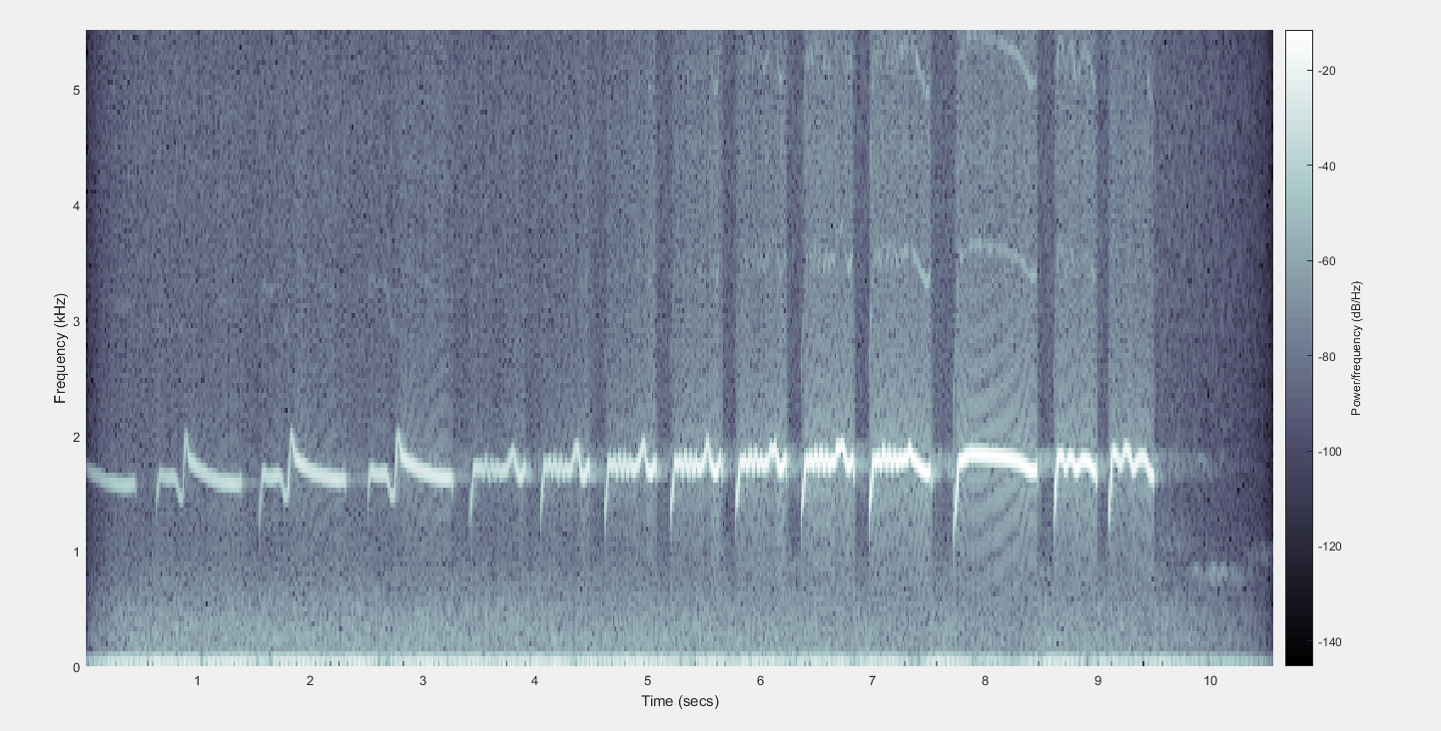
\includegraphics[width=90mm]{formants}
\caption{Formant trajectories are the white, semi-horizontal bars distinguishable from the spectrogram representation of an acoustic signal.}
\label{fig_formants}
\end{figure}
\par Now, assume that the signal can be approximated using a Linear Predictive Coding approach of $p$-th order, i.e. $\hat{\V{x}} = \sum_{k=1}^pa_k\V{x}_{t-k}$. Then, the error at each time $\V{e}_t$ between the original signal and a $p$-th order approximation is given by: 
\begin{align*}
\V{e} = \V{x} - \hat{\V{x}} = \V{x} - \sum_{k=1}^p{a_k \V{x}_{t-k}}
\end{align*} 
\par By taking the z-transform of this expression, we obtain:
\begin{align*}
\mathcal{Z}\{\V{e}\} &= \mathcal{Z}\{\V{x} - \sum_{k=1}^p{a_k \V{x}_{t-k}}\}\\
E(z) &= X(z)(1-\sum_{k=1}^p{a_k z^{-k}})\\
E(z) &= X(z)A(z)\\
\implies X(z) &= \frac{E(z)}{A(z)}
\end{align*}
\par Remark that $A(z)$ is still specified by the LPC coefficients, and thus $X(z)$, a frequency domain representation of the time signal $\V{x}$, now depends directly on the LPC coefficients \cite{Hosom2006}. The poles of the above function come in complex pairs, and are given by the roots $z_i = r_ie^{\theta_i}$ of $A(z)$. The formants in Hertz and their corresponding 3-dB bandwidth are given by \cite{Snell1993,Mathworks2015}:
\begin{align*}
F_i &= \frac{f_s}{2\pi}\theta_i \text{Hz}\\
B_i &= -\frac{f_s}{\pi}\log{(r_i)} \text{Hz}
\end{align*}
\par The bandwidth is a metric to choose how distinguishing each formant is, and represents the width of each formant peak in the frequency domain. Narrower peaks represent more distinguishing formants. 
\par Other approaches to estimate formants focus on finding different ways of estimating the LPC coefficients. For example, \cite{Darch,Araujo1998} propose calculating the LPC coefficients from a spectral envelope sampled exclusively at critical frequencies in the Mel-scale.
\par As discussed in section \ref{birdsong_review}, birdsong and human speech have been found to be very similar sounds. Given that there is a broad literature in formant sequences being used as features for human speech, using them for birdsong modelling could prove useful. For example, \cite{Ferragne2010} used formant trajectories to show the phonetic differences of 13 different British accents. In \cite{Holmes1895}, the authors used formants to classify utterances of digits in English and compare the results against other feature extraction techniques (such as cepstral features). Finally, formants were also used for vowel sounds classification in \cite{markel1976}.

\subsection{Information geometry} \label{subsection_infgeom}
The framework of Information Geometry aims at applying tools from Differential Geometry to Probability Theory \cite{Wang2009}. It assumes that each object of study belongs to a point in a Riemannian manifold, and then proceeds to define similarity metrics between these points.
\par The main motivation of this framework is to map objects into symbols that can be compared. In the domain of acoustic signals, this means to be able to build statistical models from a signal and then define a similarity metric between these.
\par The authors of \cite{Cont2011} define a framework for the analysis of acoustic signals using Information Geometry. They discuss, for example, how sequences of features (such as MFCCs) can be used to build an exponential probability distribution and how clustering (in particular, centroid computation) and model comparison can be performed over this distribution, rather than the raw features. They also apply this framework to automatically segment audio files by detecting pattern changes in the input signal.
\par Even though Information Geometry has been studied mostly for parametric families of probability distributions \cite{Amari2001}, the key concept of having a structure that summarises the information of our objects of study and then define a similarity metric between them can be retaken for other classes of models. Learning non-parametric probability distributions can be done by Kernel Density Estimation \cite{Goodall2008}, which takes a weights a combination of Kernel functions as a probability distribution; other structures, such as Hidden Markov Models \cite{Chou2008,Muda2010,Hsieh2009,Wielgat2012}, have been broadly used in the Machine Learning community to model the distribution and shape of audio sequences over time. Building these objects as an intermediate step could prove useful to construct similarity matrices as detailed in section \ref{general_pipeline}, if the right metric is defined.

\section{Metrics}\label{metrics_review}
In this section, we list and discuss some similarity measures that have proven to be useful in the literature. In particular, we focus on three groups of metrics: those between points in a vector space, those between probability densities, and those between other statistical models, such as Gaussian Mixture Models and Hidden Markov Models. The main goal is to introduce a discussion about the different contexts in which similarity measures can be used, remarking the differences between them.

\subsection{Distance between two vectors}\label{subsection_eucdist}
These metrics arise from considering two points $\V{x, y}$ as members of the same normed vector space $V$ of dimension $n$, i.e. $\V{x,y} \in V$. In the domain of Machine Learning, we can find the distance between two feature vectors by using any of the following:
\begin{definition}{Manhattan Distance.} \label{def_manhattan}
Also called City-Block distance, this metric is defined as:
\begin{align*}
d_{\text{Manhattan}}(\V{x}, \V{y}) = \sum_{i=1}^n\abs{x_i-y_i}
\end{align*}
\end{definition}
\par This distance can be interpreted as sum of all axis-wise distances between the vectors.
\begin{definition}{Euclidean distance.} \label{def_euclidean}
This is the most widespread definition of distance, given by:
\begin{align*}
d_{\text{Euclidean}}(\V{x}, \V{y}) &= \sqrt{\sum_{i=1}^n(x_i-y_i)^2}\\
&= \sqrt{\norm{\V{x}-\V{y}}}
\end{align*}
\end{definition}
\par Both definitions above can be generalised into the Minkowski distance, given by:
\begin{definition}{Minkowski distance.} \label{def_minkowski}
\begin{align*}
d_{p}(\V{x}, \V{y}) = (\sum_{i=1}^n(x_i-y_i)^{p})^{1/p}, p\in\mathbb{N}
\end{align*}
\end{definition}
\par Where the Manhattan and Euclidean distances correspond to the cases $p=1$ and $p=2$, respectively.
\par From a Linear Algebra perspective, the three definitions above can also be seen as the p-norm of the vector $\V{x}-\V{y}$, where the p-norm is given by:
\begin{definition}{$p$-norm.} \label{def_pnorm}
\begin{align*}
\norm{\V{x}}_p = (\sum_{i=1}^px_i^p)^{1/p}
\end{align*}
\end{definition}
\par Now assume that are interested in computing the pairwise distance of a set $H$ of a vector space $V$, with $H \subset V$, and that we find the smallest hyper-ellipsoid $E$ that encloses $H$. Then, it is possible that $H$ is non-spherical. This can be understood in two senses: one is that the diameter of at least one axis $x_i$ is different to the rest; the second one is that the resulting hyper-ellipsoid might be slanted with respect to at least one axis $x_i$, i.e. that  $E$ is not symmetrical with respect to all axes. See figure \ref{fig_ellipse} for a depiction of this scenario.
\begin{figure}[t]
\centering
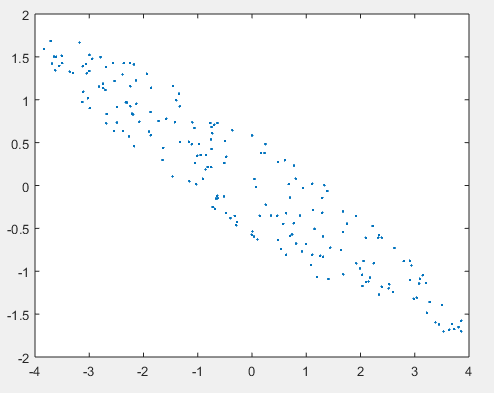
\includegraphics[width=50mm]{ellipse}
\caption{Artificial data with two correlated variables with different standard deviations.}
\label{fig_ellipse}
\end{figure}
\par The situations above describe data that has correlated variables occupying ranges of different length. In this case, computing pairwise distances using any of the methods described above could be uninformative, due to distances from larger axes diminishing the contribution of the smaller ones. As a consequence, a means of computing distance that would consider these variances in data was proposed by Mahalanobis in 1936 \cite{Bellet2013}.

\begin{definition}{Mahalanobis distance.} \label{def_mahalanobis}
Let $S$ be the covariance matrix of the set $H$ subset of a vector space $V$. Then, the Mahalanobis distance between two points $\V{x,y}\in H$ is given by:
\begin{align*}
d_{M}(\V{x}, \V{y}) = \sqrt{(\V{x}-\V{y})^TS^{-1}(\V{x}-\V{y})}
\end{align*}
\end{definition}

\par In this case, the matrix $S^{-1}$ can be seen as a linear transformation that "decorrelates" the data and then calculates the Euclidean distance as in definition \ref{def_euclidean}. 

\subsection{Distance between two probability distributions}\label{subsection_pdfdist}
In this subsection, we present distance metrics for probability distributions. We remark that the main goal of these methods is to quantify the similarity of two statistical objects, rather than two elements of a vector space. As a consequence, there is a change of focus in how we compute these distances: rather than manipulating the definition of the norm of a vector, we use statistical and information-theoretic foundations to define a similarity metric. 
\begin{definition}{Symmetric Kullback-Leibler Divergence.} \label{def_skld1}
Let $P(x), Q(x)$ be two probability distributions defined over the same domain. Then, the Symmetric KL-Divergence between $P$ and $Q$ is given by:
\begin{align*}
d_{\text{SKLD}}\infdiv{P}{Q} = \frac{d_{KL}\infdiv{P}{Q} + d_{KL}\infdiv{Q}{P}}{2}
\end{align*}
\end{definition}
\par where $d_{KL}\infdiv{P}{Q}$ is the KL-Divergence of $Q$ from $P$, which is defined as:
\begin{definition}{Kullback-Leibler Divergence.} \label{def_kld1}
Let $P(x), Q(x)$ be two probability distributions defined over the same domain. Then, the KL-Divergence of $Q$ from $P$ is given by:
\begin{align*}
d_{KL}\infdiv{P}{Q} = \int_{-\infty}^{\infty}P(x)\log{(\frac{P(x)}{Q(x)})}dx
\end{align*}
\end{definition}
\par The above is only defined for distributions satisfying $Q(x) = 0 \implies P(x) = 0$. It can now be seen that the SKLD is just a procedure to add the symmetry property to the KL-Divergence. It can also be seen that the KL-Divergence already satisfies the rest of the properties from definition \ref{def_metric}, and that they are inherited by the SKLD \cite{Hershey2007}. 
\par Intuitively, the KL-Divergence can be understood as a relative entropy measure \cite{Divergence2008}, i.e. how much information can we lose if we let $Q$ approximate $P$? By taking the average, we are also measuring the converse (letting $P$ approximate $Q$) and then re-scaling the result.
\begin{definition}{Hellinger distance.} \label{def_hellinger1}
The Hellinger distance between two discrete probability distributions $P, Q$ is given by:
\begin{align*}
h(P, Q) &= \frac{1}{\sqrt{2}}\norm{P-Q}_2\\
&= \sqrt{\sum_{i}(\sqrt{P_i}-\sqrt{Q_i})^2}
\end{align*}
\end{definition}

\begin{definition}{Bhattacharyya coefficient.} \label{def_bhattacharyyacoef}
The Bhattacharyya coefficient between two discrete distributions $P, Q$ is given by:
\begin{align*}
\rho(P, Q) = \sum_i{\sqrt{P_iQ_i}}
\end{align*}
\par This can be interpreted geometrically as the cosine of the angle $\theta$ between the vectors \begin{align*}
P' = \begin{pmatrix}\sqrt{P_1}&\sqrt{P_2}&...&\sqrt{P_N}\end{pmatrix}\\
Q' = \begin{pmatrix}\sqrt{Q_1}&\sqrt{Q_2}&...&\sqrt{Q_N}\end{pmatrix}
\end{align*}
\end{definition}
\par Whenever both distributions are equal, $\rho(P, P) = 1 \implies \theta = 0$, whereas completely disjoint distributions $P, R$ yield $\rho(P, R) = 0 \implies \theta = 1$. The Bhattacharyya coefficient serves to define the Bhattacharyya distance:
\begin{definition}{Bhattacharyya distance.} \label{def_bhattacharyya}
\begin{align*}
d_B(P, Q) = \sqrt{1 - \rho(P, Q)}
\end{align*}
\end{definition}

\par The last metric we present works for unidimensional distributions, and is defined below.
\begin{definition}{Kolmogorov-Smirnov two-sample distance.} \label{def_ks2s}
\begin{align*}
D_{KS}(P, Q) = \sup_{x}\abs{P(x)-Q(x)}
\end{align*}
\end{definition}
\par This distance can be interpreted as the maximum vertical distance both distributions at any point $x$, and is widely used as a statistical test to prove whether two empirical distributions differ \cite{KSMathworks2015}.

\subsection{Distance between other statistical models}\label{subsection_models}
In this subsection we consider the problem of measuring similarity between other statistical models. For the sake of illustrating the scenario, we will be focusing on a single family of models: Hidden Markov Models (HMMs). Although there is a wide variety of statistical models, focusing on one can be illustrative enough to show the arising challenges. A broader discussion on HMMs and their applications is given in chapter \ref{chapter_hmms}.
\par The main point to raise in this review is that defining a measure for a statistical model requires knowing and establishing conditions on what similarity \emph{means} in the context of the model. For example, are two HMMs comparable only if they have the same number of states? How should distance metrics make use of the parameters of the model? How does the metric deal with inherent issues of the model, such as identifiability? There exists no clear, established answer to any of these.
\par Nevertheless, some work has been done to define similarity measures for HMMs with available frameworks. For example, the authors of \cite{Lyngs1999} define a distance metric based on co-emission probability, i.e. based on the probability that two HMMs $h_1, h_2$ independently generate the same sequence of observations $s$. The co-emission probability is given by:
\begin{align*}
A(h_1, h_2) = \sum_{s\in \Sigma^*}P_{h_1}(s)P_{h_2}(s)
\end{align*}
\par Then, a similarity measure between $h_1, h_2$ is given by:
\begin{align*}
S_1(h_1, h_2) = \frac{A(h_1, h_2)}{\sqrt{A(h_1, h_1)A(h_2, h_2)}}
\end{align*}
\par Additionally, in \cite{Bahlmann2001}, the authors use the Bayes Probability Error to define a metric between two models. 
\begin{definition}{Bayes Probability Error.} \label{def_bpe}
The Bayes Probability Error between two densities $p_1(\V{x}), p_2(\V{x})$ is given by:
\begin{align*}
P_e(p_1(\V{x}), p_2(\V{x})) = \int_\V{x}\min{\{\pi_1p_1(\V{x}), \pi_2p_2(\V{x})\}}d\V{x}
\end{align*}
\end{definition}
\par The Bayes Probability Error can be understood as "the area of overlap of two densities $p_1, p_2$ with priors $\pi_1, \pi_2$ under the restriction $\pi_1+\pi_2 = 1$". The authors train handwriting recognition HMMs and then define their misclassification error in terms of their similarity metric, which is defined as:
\begin{align*}
D(h_1, h_2) = 1 - 2P_e{(\mathcal{N}(h_1, \V{x}), \mathcal{N}(h_2, \V{x}))}
\end{align*}
\par Where $P_e{(\mathcal{N}(h_1, \V{x}), \mathcal{N}(h_2, \V{x}))}$ represents the Bayes Probability Error over the Gaussian emission probabilities in the HMMs. Although this definition only considers Gaussian emission probabilities, it can be adapted to other variants of HMMs by using the corresponding emission densities to compute $P_e$ accordingly.
\par A third distance measure was proposed in \cite{Juang1985}. Let $h_1, h_2$ be two discrete HMMs with empirical emission distributions given by $\V{B}_1, \V{B}_2$. Then, an HMM distance metric is given by:
\begin{align*}
d(h_1, h_2) = \norm{\V{B}_1 - \V{B}_2}
\end{align*}
\par This metric has the disadvantage of not taking into account any of the other parameters in the HMMs. Furthermore, it is only defined for discrete-observation HMMs.
\par To conclude, we review that HMM similarity is still an open problem, and that, in general, statistical model similarity poses several challenges that are inherent to the model itself, hence reducing the possibilities of finding a cross-model metric. In the case of HMMs, different approaches have used their parameters in different fashions to define metrics, some opting to not use all the parameters in their definition. A broader discussion on this is presented in chapter \ref{chapter_hmms}.

\section{Building relational structures}\label{algorithms_review}
In this section, we present an overview of algorithms to build relational structures from distance matrices (unless a different input is stated). The goal is to give an outline of the different general approaches that have been presented in the literature, and what they were aiming at. We first introduce traditional approaches to clustering; then, we present more novel approaches to the same problem; finally, we introduce algorithms useful to detect communities in complex graphs.

\subsection{K-means algorithm} \label{subsection_kmeans}
The first algorithm that we cover is K-means. This is an iterative descent algorithm that partitions a purely quantitative set $X$ of $M$ feature vectors into $K$ clusters \cite{hastie2008}. The procedure is divided in two stages: we first choose centroids $\{C_i\}$ (at random for initialisation, and then by finding the mean vector of every cluster) and then create new clusters by assigning each data point to the cluster with the closest centroid $C_i$ (in terms of the Euclidean distance). This is repeated until the clusters stop changing. Pseudocode for this procedure is given in algorithm \ref{alg_kmeans}.
\begin{algorithm}
\begin{algorithmic}[1]
\label{alg_kmeans}
\Function{kmeans}{$X, K$}
\State choose $K$ points at random from $X$
\Repeat
\ForAll{$x_i$}
    \ForAll{$c_j$}
        \State $d(i,j) = \norm{x_i - c_j}$
    \EndFor  
    \State $j' = \argmin_j{d(i, :)}$\Comment{choose centroid with minimum distance}
    \State $C(j')$.add($x_i$)
\EndFor
\ForAll{$C(j')$}
    \State set $c_j \gets \frac{1}{\abs{C(j')}}\sum_{x_i \in C(j')}{x_i}$\Comment{recompute centroids}
\EndFor  
\Until{convergence}
\EndFunction
\caption{The K-means algorithm}
\end{algorithmic}
\end{algorithm}
\par Despite its simplicity, K-means has some disadvantages, such as being sensitive to the order of presentation of data, e.g. if two centroids are equally apart from a single data point $x_i$, then it will be assigned to the cluster that is presented last. Moreover, K-means only gives a snapshot of the data at a specific point in time - it doesn't describe how the links are formed over time. 

\subsection{Agglomerative hierarchical clustering} \label{subsection_hier}
This is one of the "traditional methods for detecting community structure" \cite{Girvan2002}, whose output is an arborescent structure created by progressively linking clusters. We begin assuming that each point in the dataset is a singleton cluster, and in each iteration we create a new cluster by merging the two closest clusters \cite{hastie2008}. We remark that the input to this algorithm is a similarity matrix (rather than feature vectors, as in K-means) and that, every time we merge a cluster, we only have to update the distances between the newly created cluster and the rest. 
\par The simplest linking technique is \emph{single linkage}, which takes the inter-cluster distance to be the one between the most similar pair, i.e. for clusters $C_1, C_2$, their single linkage distance is given by:
\begin{align*}
d_{SL} = \min_{x_i\in C_1, x_i'\in C_2}{d_{i,i'}}
\end{align*}
\par The procedure stops when there is only one cluster containing all data. The output of hierarchical clustering is a list of triples $(C_i, C_i', d_{i,i'})$ that can be seen as records of clusters that were merged together, and how afar they were from each other. This list of tuples can then be visualised as a dendrogram \cite{HAGMathworks}, which is the tree-like structure depicted in figure \ref{fig_hag}. It is important to notice that agglomerative approaches possess a \emph{monotonicity} property: "the dissimilarity between merged clusters is monotone increasing with the level of the merger". If this were not the case, a dendrogram representation of the data would not be possible \cite{hastie2008} - as it is the case for some divisive approaches, discussed in subsection \ref{subsection_divisive}. A broader discussion of this technique and other linking strategies can be found in chapter \ref{chapter_hmms}.
\par As opposed to K-means, hierarchical clustering shows an evolution of clusters over time, so it can be used to model both, how communities cluster together as times flows, but also take a closer look at how a community looked at a specific moment in time.
\begin{figure}[t]
\centering
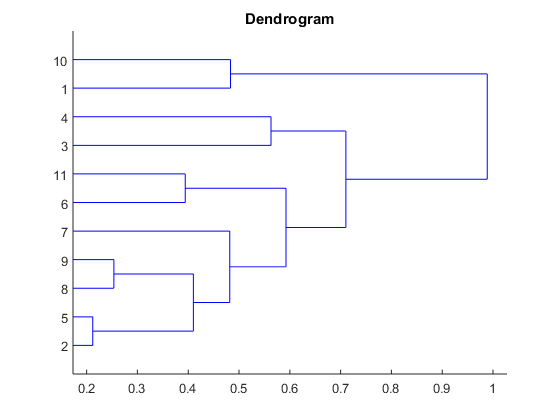
\includegraphics[width=80mm]{dendrogram}
\caption{A dendrogram with 11 leaves. The horizontal axis is the distance between the merged clusters; the vertical axis is the identifier of the leaves.}
\label{fig_hag}
\end{figure}

The traditional method for detecting community structure in networks such as that depicted in Fig. 1 is
hierarchical clustering. One first calculates a weightWij for every
pair i,j of vertices in the network, which represents in some sense
how closely connected the vertices are.

\subsection{Divisive hierarchical clustering} \label{subsection_divisive}
This approach can be seen as the counterpart of agglomerative clustering: rather than starting with $\abs{X}$ clusters, the algorithm considers the whole set $X$ as a single cluster and then splits it iteratively. Some results have shown that this paradigm can produce more accurate results in a shorter amount of time than agglomerative clustering, although there has not been as much research about it \cite{Manning2009}.  
\par In the simplest case, K-means is applied iteratively to the dataset, i.e. we partition the input cluster into 2 subclusters using $K=2$, and then repeat this procedure for each cluster. However, this approach lacks the monotonicity property described in subsection \ref{subsection_hier}, and hence a consistent dendrogram representation is not guaranteed \cite{hastie2008}.
\par Further approaches to divisive clustering include the one proposed by Macnaughton Smith in 1965 \cite{hastie2008}, which proceeds as follows: at each iteration, choose the element from input cluster $G$ whose average distance from the rest $G' = G - \{x_i\}$ is largest. The average dissimilarity of $x_i$ with respect to $G'$ is given by:
\begin{align*}
\bar{d}_{G'}(x_i) = \frac{1}{\abs{G'}}\sum_{i'\in G'} d_{i,i'}
\end{align*}
\par This is the seed of a new cluster, $H$. For each successive step, add to $H$ the element $x_i$ such that:
\begin{align*}
\argmax_{x_i \in X} \bar{d}_H(x_i) - \bar{d}_{G-\{x_i\}}
\end{align*}
\par This continues until the expression above becomes negative, in which case the algorithm is now applied recursively to $G$ and $H$. This means that there is no other element in $G$ that is closer to $H$ in average \cite{hastie2008}. A broader discussion of divisive hierarchical clustering splitting techniques can be found in \cite{.2006};

\subsection{Girvan-Newman algorithm} \label{subsection_gn}
This algorithm was first proposed in \cite{Girvan2002}, and focuses on analysing the edges of the network (rather than the vertices). In particular the algorithm chooses edges that lie "between" clusters-to-be, and removes them. This metric is called \emph{edge betweenness}, and is defined as "the number of shortest paths between pairs of vertices that run along it" \cite{Girvan2002}. Edges $e\in E$ with greater betweenness are likely to connect communities, and thus removing them encourages the partitioning of vertices \cite{Lu2012}.
\begin{algorithm}
\begin{algorithmic}[1]
\label{alg_gn}
\Function{gncommunity}{$X, K$}
\Repeat
\ForAll{edges $e \in E$}
    \State Calculate betweenness $b(e)$
\EndFor
\State remove $\argmax_e{b(e)}$
\Until{no edges have been affected by the last removal}
\EndFunction
\caption{The GN algorithm for community detection.}
\end{algorithmic}
\end{algorithm}
\par The main disadvantage of this approach is that it does not handle weighted graphs, thus distance matrices cannot be used to find inner communities.

\subsection{Soft-partitioning} \label{subsection_softpart}
All the approaches presented until now assume that a single data point can only belong to one cluster or community. However, it is often the case that communities overlap, i.e. that there are at least two clusters $C_i, C_j$ such that $C_i \cap C_j \neq \emptyset$. An approach to solve this problem is proposed in \cite{Psorakis2010}, and relies on matrix factorisation techniques.
\par Let $\V{V}$ be a matrix of interactions where $v_{i,j}$ denotes the number of interactions between objects $x_i, x_j$. Then, we can model $\hat{\V{V}}$ as the product of two rank $K$ matrices $\V{W} \in \mathbb{R}_+^{N \times K}, \V{H}\in \mathbb{R}_+^{K \times N}$, i.e. $\hat{\V{V}} = \V{WH}$, where $K$ is the number of hidden communities in the network. The product $w_i^Th_j$ can be seen as the \emph{expected number of participations} two individuales $x_i, x_j$ are expected to have - their mutual participation \cite{Psorakis2010}. However, the number of communities $K$ is usually unknown. The authors address this issue by placing automatic relevance determination priors $\V{B} = \text{diag}(\beta_k)$ on the latent variables $w_{ik}, h_{k, j}$ using a Gamma distribution with parameters $a, b$\cite{Psorakis2010a}.
\par The parameters of this model can be found iteratively via algorithm \ref{alg_nmf} from \cite{Psorakis2010a}:
\begin{algorithm}
\begin{algorithmic}[1]
\label{alg_nmf}
\Function{nmf}{$V, K_0, a, b$}
\Repeat
    \State $\V{H} \gets \frac{\V{H}}{\V{W}^T\V{1}+\V{BH}}\V{W}^T\V{\frac{\V{V}}{\V{WH}}}$
    \State $\V{W} \gets \frac{\V{W}}{\V{1}\V{H}^T+\V{WB}}\V{\frac{\V{V}}{\V{WH}}}\V{H}^T$
    \State $\beta_k \gets \frac{N-a-1}{1/2(\sum_i{w_{ik}^2} + \sum_j{h_{kj}^2})} + b$
\Until{$n_iter$}
$K_f \gets $ number of non-zero columns of $\V{W}$ or rows of $\V{H}$
\State \textbf{return} $\V{W}_f \in \mathbb{R}_+^{N\times K_f}, \V{H}_f\in\mathbb{R}_+^{K_f\times N}$
\EndFunction
\caption{The GN algorithm for community detection.}
\end{algorithmic}
\end{algorithm}
\par Details on the derivation of these update rules can be found in \cite{Psorakis2010a,Psorakis2010a}. 
\par The main advantage of this method is that it accounts for overlapping communities and finds an approach that works well over weighted graphs (an aspect lacking from the approach in subsection \ref{subsection_gn}. Work to incorporate other factors in community detection, such as time and geographical dynamics is under way \cite{Psorakis2010}.

\section{Conclusion}
In this chapter we introduced a general pipeline to build relational structures, with three main processes: feature extraction, distance matrix computation, and cluster generation. Then, we described general aspects of birdsong that could be useful to choose appropriate techniques for later stages of the process. For each of the subsequent sections, we presented several techniques to "fill in the gaps" of the general pipeline described in section \ref{general_pipeline}.
\par From section \ref{features_review}, we learned that one technique that is useful to model vocal sounds are formant. Although not much research of formants applied to birdsong has been done, this project could set some preliminary results to test whether they would be a faithful representation of birdsong data. Formants and a signal analysis review to fully understand them are covered in chapter \ref{chapter_formants}.
\par Additionally, in section \ref{features_review}, we also learned that using an intermediate statistical model, such as a probability distribution or a Hidden Markov Model, can serve to summarise the content and structure of data. In \ref{chapter_hmms}, we further discuss the details on how to build this kind of models and expand the review of similarity metrics from \ref{metrics_review}.
\par Then, hierarchical clustering is retaken in chapter \ref{chapter_hmms} as well. This approach can be useful to model dynamics in communities and clusters, especially in bird species, discovering structures under specific lifetimes is relevant. 
\par To conclude, we have seen that although there is a limited amount of research on birdsong community detection, it can be quite approachable by filling the gaps of a generic pipeline - this means that this review also serves to set a basis for work to be done beyond this dissertation.
\end{document}